\documentclass{article}
\usepackage[utf8]{inputenc}
\usepackage{graphicx}
\usepackage[margin=1in]{geometry}
\usepackage[backend=bibtex,style=ieee]{biblatex}
\addbibresource{textmining_julki092.bib}
\newcommand{\HRule}[1]{\rule{\linewidth}{#1}}

\begin{document}
	
	\title{\textsc{732A92 Text Mining} \\ [2.0cm]
		\HRule{0.5pt} \\
		\LARGE \textbf{\uppercase{Classifying Stock Price Movements based on 8-K SEC filings}}
		\HRule{2pt} \\ [0.5cm]
		\normalsize \today \vspace*{5\baselineskip}}
	
	\date{}
	
	\author{
		Name: Julius Kittler \\ 
		Student ID: julki092 \\ 
		Link\"{o}ping University}
	
	\maketitle
	\newpage
	
	\begin{abstract}
		
		For over a century, fingerprints have been an undisputed
		personal identifier.  Recent court rulings have sparked
		interest in verifying unique
	\end{abstract}

	\newpage
	\tableofcontents
	\newpage
	\listoffigures
	\newpage

	\section{Introduction}
	
	Forecasting stock prices has been a relevant problem since the existence of publicly traded companies. Today, it is a more relevant problem than ever before because we have the technological infrastructure to build automatic trading systems and thereby put our forecasts to practice. We can not only obtain massive amounts of data relevant for forecasts via APIs but also execute trades via APIs. With commission free trading having become the industry standard in the U.S., the latter services are even offered for free, for instance by the commission free algorithmic trading API Alpaca \cite{noauthor_alpaca_nodate}. 
	
	This text mining project aims to explore whether filings of the U.S. Securities and Exchange Commission (SEC) can be used to classify if the price of a stock will decrease, remain unchanged or increase. The results will be evaluated critically from the perspective of a trader, with the question in mind whether the classifications could actually be put to practice in an automatic trading system.
	

	\subsection{SEC Filings}
	
	The SEC is a government agency in the United States with the mission to "protect investors, maintain fair, orderly, and efficient markets, and facilitate capital formation" \cite{noauthor_sec.gov_nodate}. An important task of the SEC is to ensure that publicly traded companies inform their shareholders and the public about their business.
	
	For instance, the SEC requires companies to publish their quarterly and annual results, and inform shareholders about certain relevant events. For each of these purposes, companies have to file specific documents. For instance, the annual report corresponds to the 10-K, the quarterly report corresponds to the 10-Q and another report for specific relevant events corresponds to the 8-K filing.
	
	Importantly, SEC filings are actively used by traders when making investment decisions. Many trading platforms such as Webull and thinkorswim also provide traders with the recent SEC filings of any tradable company (along with other information such as fundamental data, news data and historical prices). SEC filings are interesting for stock price forecasting because they are standardized, publicly accessible for free and because they contain relevant, objective and generally accurate information.
	
	
	\subsection{8-K Filings}
	
	Companies need to publish an 8-K filing for major events relevant for their business. Such events might be a change in the board of directors, a delisting from a stock exchange and a merger or acquisition \cite{noauthor_sec.gov_nodate-1}. Importantly, 8-K filings are generally due within four business days after the event \cite{kenton_8-k_nodate}. 
	
	Because 8-K filing correspond to major events for the company and because they need to be published shortly after an event occurred, 8-K filings seem interesting for predicting short-term volatility in the stock market. Moreover, the important information in 8-K filings is generally represented in form of text data, whereas other filings such as the annual report often focus on numerical data represented in tabular form.
	
	\textbf{TODO: EXAMPLE}

	\begin{figure}[h]
		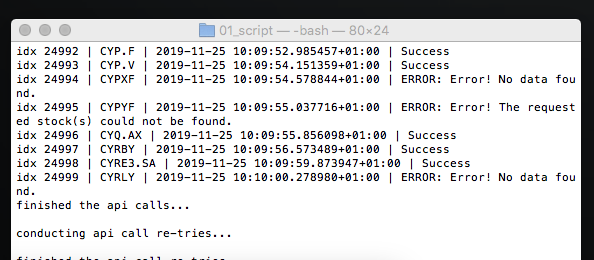
\includegraphics[width=\linewidth]{img/test.png}
		\caption{A boat.}
		\label{fig:boat1}
	\end{figure}
	
	Figure \ref{fig:boat1} shows a boat.
	
	
	\subsection{Research Questions}
	
	There are mainly three research questions that this report aims to address. The focus is not only on the stock price classification itself but importantly also on understanding how the model works. Assuming that we do not know much about SEC filings, we would like the model to give insights about how it is using the text data of the SEC filings for the classification and in which cases the model is more or less reliable. 
	
	\begin{enumerate}
		\item Can we successfully forecast stock prices based on 8-K filings? If so, how well?
		\item Which text features are most important when forecasting stock prices based on 8-K filings?
		\item In which scenario do the forecasts perform best (e.g. type of the 8-K filing, industry of the company, other metrics of the company)?
	\end{enumerate}
	

	\section{Theory}
	
	Previous work in predicting stock prices with 8-K filings.
	
	\subsection{Stock Price Forecasting in General}
	tbd 
	
	\subsection{Stock Price Forecasting with Text Data}
	tbd
	
	\subsection{State of the Art Classification with Text Data}
	tbd

	\section{Data}
	
	\subsection{Retrieval}
	
	Data sources, Time period, Exchange Market, Resolution
	
	\subsection{Processing}
	
	\subsection{Descriptive Statistics}
	
	\subsubsection{General}
	
	\subsubsection{Target Variable}
	
	\subsubsection{Feature Variables}
	

	\section{Method}
	
	\subsection{Evaluation Metric}
	
	\subsection{Baseline Models}
	
	\subsection{Advanced Models}
	
	\subsection{Hyperparameter Tuning}
	
	Train vs. test
	
	\subsection{Feature Relevance}
	
	\section{Results}
	
	
	
	\section{Discussion}
	
	\section{Conclusion}
	
	\section{References}
	
	\cite{radioactivedecay2}
	\cite{DLS1}  

	
\printbibliography
\end{document}
